\chapter{Aditional plots}

\section{Pre-selection kinematic variables} \label{app:presel_plots}

Figures~\ref{fig:input_vars_3l_xsec}, \ref{fig:input_vars_2lss_xsec_mumu} and~\ref{fig:input_vars_2lss_xsec_emu} show the distributions of some relevant kinematic variables, normalized to the cross section of the respective processes and to the integrated luminosity.
\newpage
\begin{figure} [!h]
  \centering
  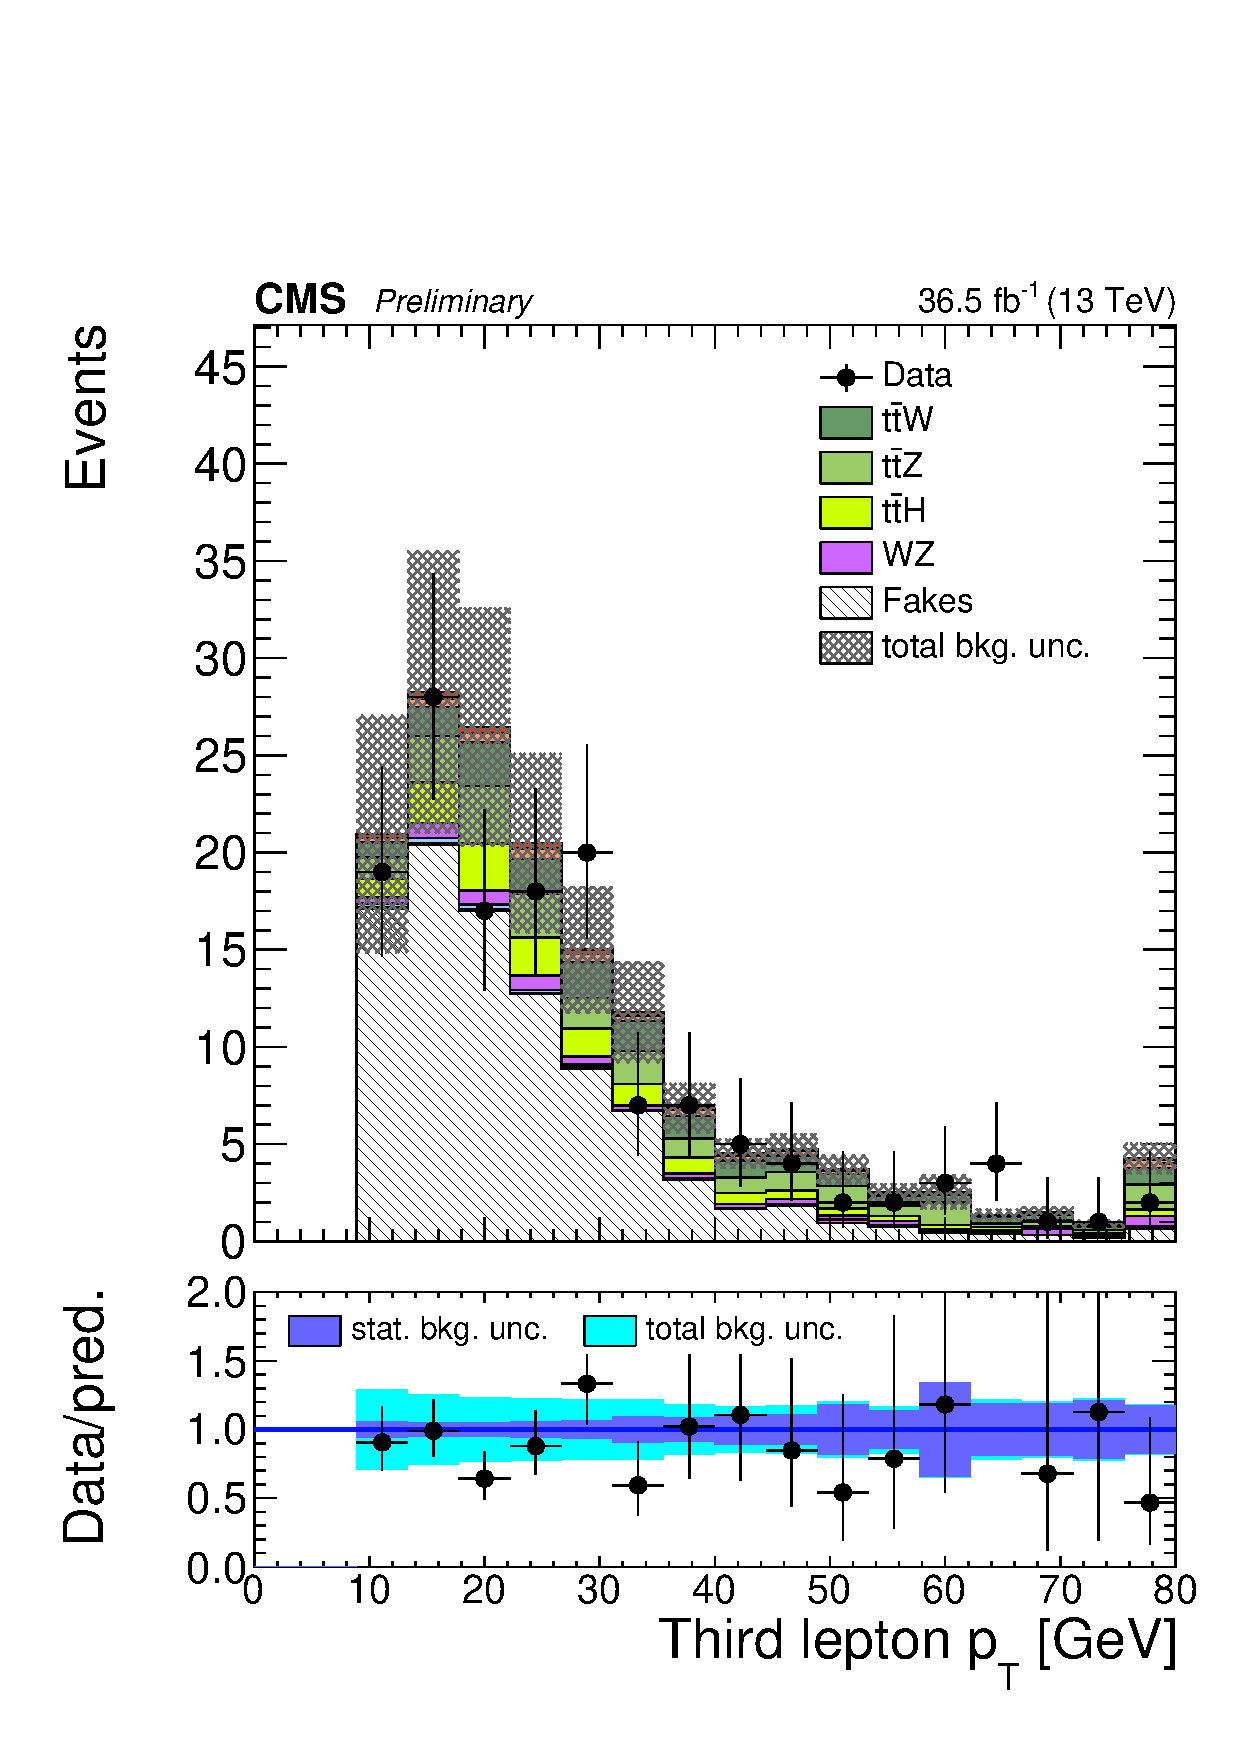
\includegraphics[width=0.26\textwidth]{3lsignal/Lep3Pt.pdf}
  \includegraphics[width=0.26\textwidth]{3lsignal/dEtaFwdJetBJet_40.pdf}
  \includegraphics[width=0.26\textwidth]{3lsignal/dEtaFwdJet2BJet_40.pdf}\\
  \includegraphics[width=0.26\textwidth]{3lsignal/dEtaFwdJetClosestLep_40.pdf} 
  \includegraphics[width=0.26\textwidth]{3lsignal/dPhiHighestPtSSPair.pdf}
  \includegraphics[width=0.26\textwidth]{3lsignal/maxEtaJet25_40.pdf}\\
  \includegraphics[width=0.26\textwidth]{3lsignal/minDRll.pdf}
  \includegraphics[width=0.26\textwidth]{3lsignal/nJet25.pdf} 
  \includegraphics[width=0.26\textwidth]{3lsignal/nJetEta1_40.pdf}\\
  \includegraphics[width=0.26\textwidth]{3lsignal/totCharge.pdf}
  \caption[Input variables to the BDT, $3l$ channel.]{Distributions of input variables to the BDT for signal discrimination, three lepton channel, normalized to their cross section and to 35.9 \fbinv.}
  \label{fig:input_vars_3l_xsec}
\end{figure}

\begin{figure} [!h]
  \centering
  \includegraphics[width=0.26\textwidth]{signalregion_2lss/mumu/Lep2Pt.pdf}
  \includegraphics[width=0.26\textwidth]{signalregion_2lss/mumu/dEtaFwdJetBJet_40.pdf}
  \includegraphics[width=0.26\textwidth]{signalregion_2lss/mumu/dEtaFwdJet2BJet_40.pdf}\\
  \includegraphics[width=0.26\textwidth]{signalregion_2lss/mumu/dEtaFwdJetClosestLep_40.pdf}
  \includegraphics[width=0.26\textwidth]{signalregion_2lss/mumu/dPhiHighestPtSSPair.pdf}
  \includegraphics[width=0.26\textwidth]{signalregion_2lss/mumu/maxEtaJet25_40.pdf}\\
  \includegraphics[width=0.26\textwidth]{signalregion_2lss/mumu/minDRll.pdf}
  \includegraphics[width=0.26\textwidth]{signalregion_2lss/mumu/nJet25.pdf} 
  \includegraphics[width=0.26\textwidth]{signalregion_2lss/mumu/nJetEta1_40.pdf}\\
  \includegraphics[width=0.26\textwidth]{signalregion_2lss/mumu/totCharge.pdf}
  \caption[Input variables to the BDT, $2lss - \mumu$ channel]{Distributions of input variables to the BDT for signal discrimination, in \mumu\ channel, normalized to their cross section and to 35.9 \fbinv.}
  \label{fig:input_vars_2lss_xsec_mumu}
\end{figure}

\begin{figure} [!h]
  \centering
  \includegraphics[width=0.26\textwidth]{signalregion_2lss/emu/Lep2Pt.pdf}
  \includegraphics[width=0.26\textwidth]{signalregion_2lss/emu/dEtaFwdJetBJet_40.pdf}
  \includegraphics[width=0.26\textwidth]{signalregion_2lss/emu/dEtaFwdJet2BJet_40.pdf}\\
  \includegraphics[width=0.26\textwidth]{signalregion_2lss/emu/dEtaFwdJetClosestLep_40.pdf} 
  \includegraphics[width=0.26\textwidth]{signalregion_2lss/emu/dPhiHighestPtSSPair.pdf}
  \includegraphics[width=0.26\textwidth]{signalregion_2lss/emu/maxEtaJet25_40.pdf}\\
  \includegraphics[width=0.26\textwidth]{signalregion_2lss/emu/minDRll.pdf}
  \includegraphics[width=0.26\textwidth]{signalregion_2lss/emu/nJet25.pdf} 
  \includegraphics[width=0.26\textwidth]{signalregion_2lss/emu/nJetEta1_40.pdf}\\
  \includegraphics[width=0.26\textwidth]{signalregion_2lss/emu/totCharge.pdf}
  \caption[Input variables to the BDT, $2lss-\emu$ channel]{Distributions of input variables to the BDT for signal discrimination, in $\emu$ channel, normalized to their cross section and to 35.9 \fbinv.}
  \label{fig:input_vars_2lss_xsec_emu}
\end{figure}

%% \begin{figure} [!h]
%%   \centering
%%   \includegraphics[width=0.22\textwidth]{signalregion_2lss/ee/Lep2Pt.pdf}
%%   \includegraphics[width=0.22\textwidth]{signalregion_2lss/ee/dEtaFwdJetBJet_40.pdf}
%%   \includegraphics[width=0.22\textwidth]{signalregion_2lss/ee/dEtaFwdJet2BJet_40.pdf}
%%   \includegraphics[width=0.22\textwidth]{signalregion_2lss/ee/dEtaFwdJetClosestLep_40.pdf} \\
%%   \includegraphics[width=0.22\textwidth]{signalregion_2lss/ee/dPhiHighestPtSSPair.pdf}
%%   \includegraphics[width=0.22\textwidth]{signalregion_2lss/ee/maxEtaJet25_40.pdf}
%%   \includegraphics[width=0.22\textwidth]{signalregion_2lss/ee/minDRll.pdf}
%%   \includegraphics[width=0.22\textwidth]{signalregion_2lss/ee/nJet25.pdf} \\
%%   \includegraphics[width=0.22\textwidth]{signalregion_2lss/ee/nJetEta1_40.pdf}
%%   \includegraphics[width=0.22\textwidth]{signalregion_2lss/ee/totCharge.pdf}
%%   \caption{Distributions of input variables to the BDT for signal discrimination, in $\ee$ channel, normalized to their cross section and to 35.9\fbinv.}
%%   \label{fig:input_vars_2lss_xsec_ee}
%% \end{figure}

\section{BDTG input variables for $2lss$ channel }

\begin{figure} [!h]
  \centering
  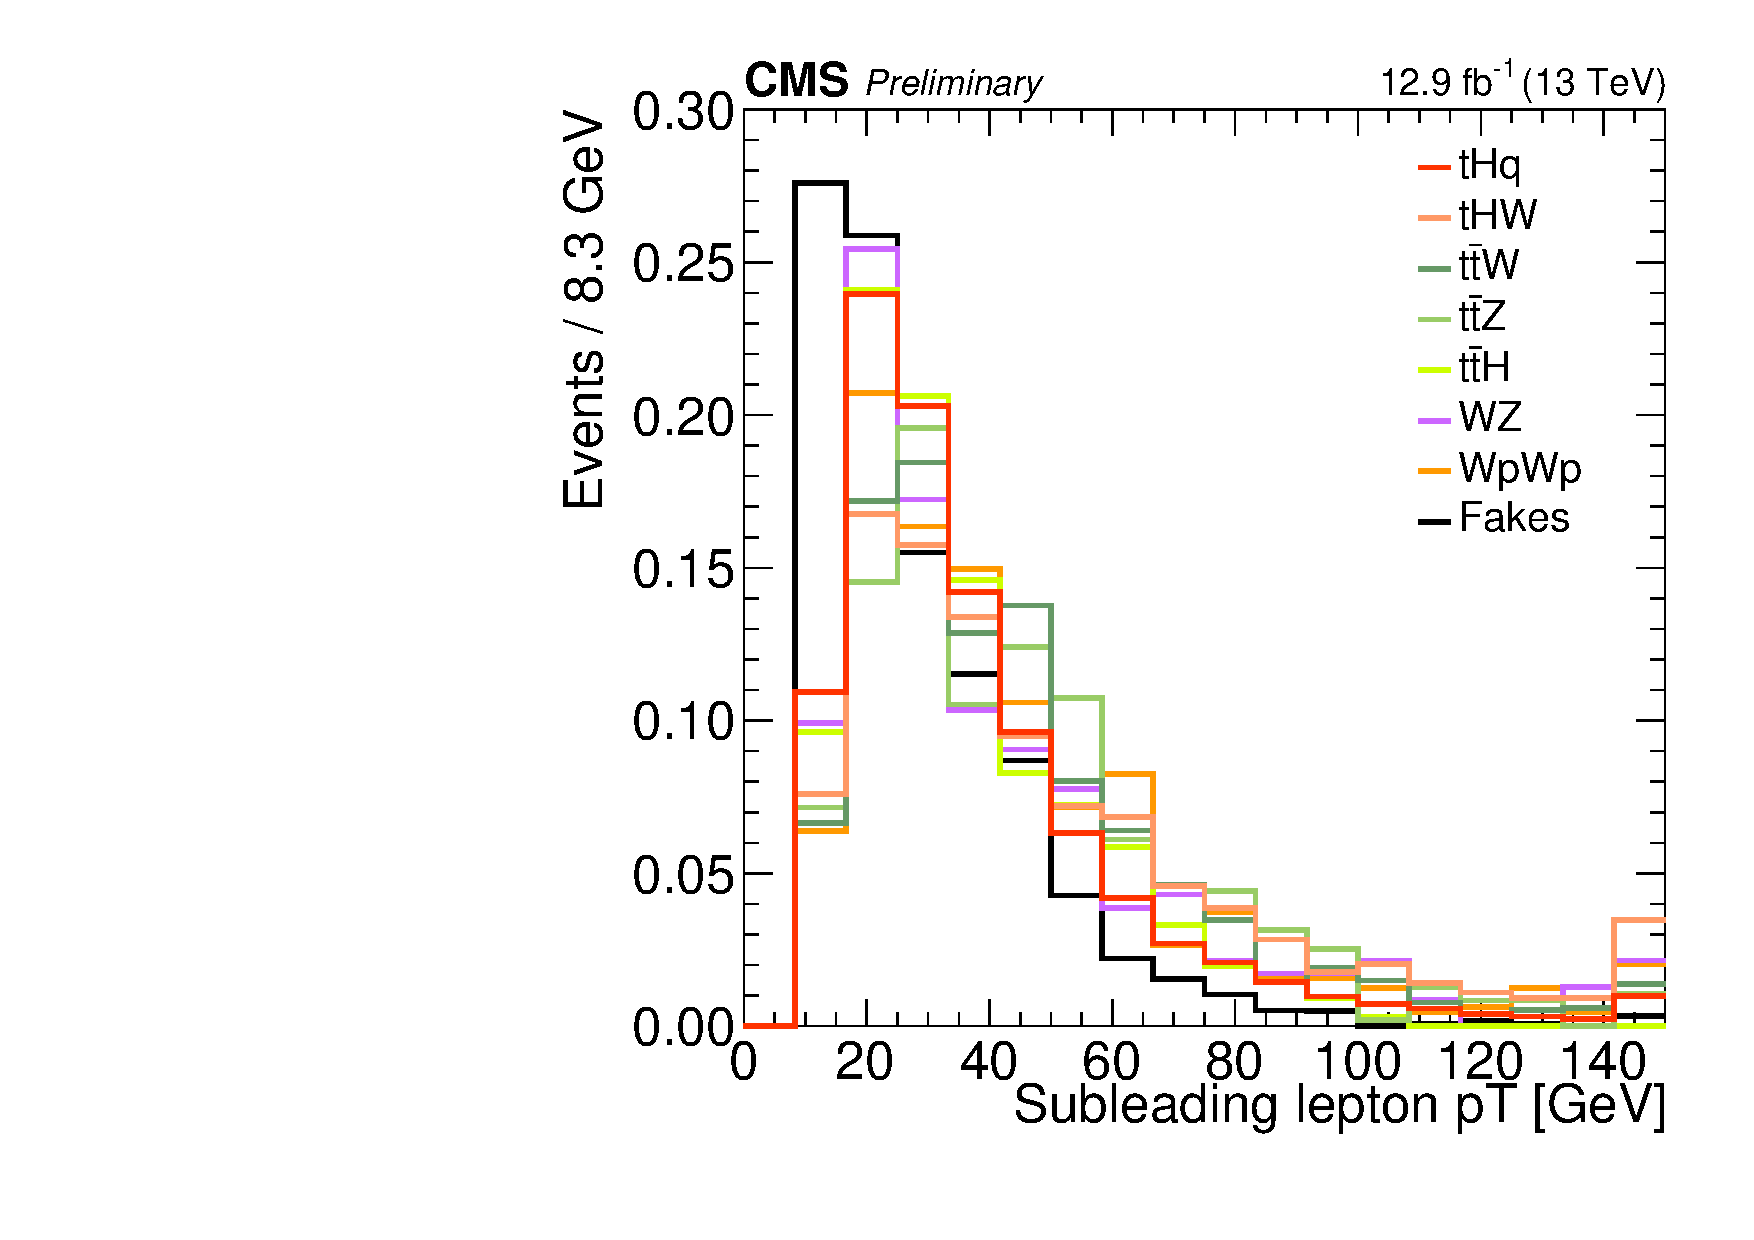
\includegraphics[width=0.32\textwidth]{Lep2Pt_mumu.pdf}
  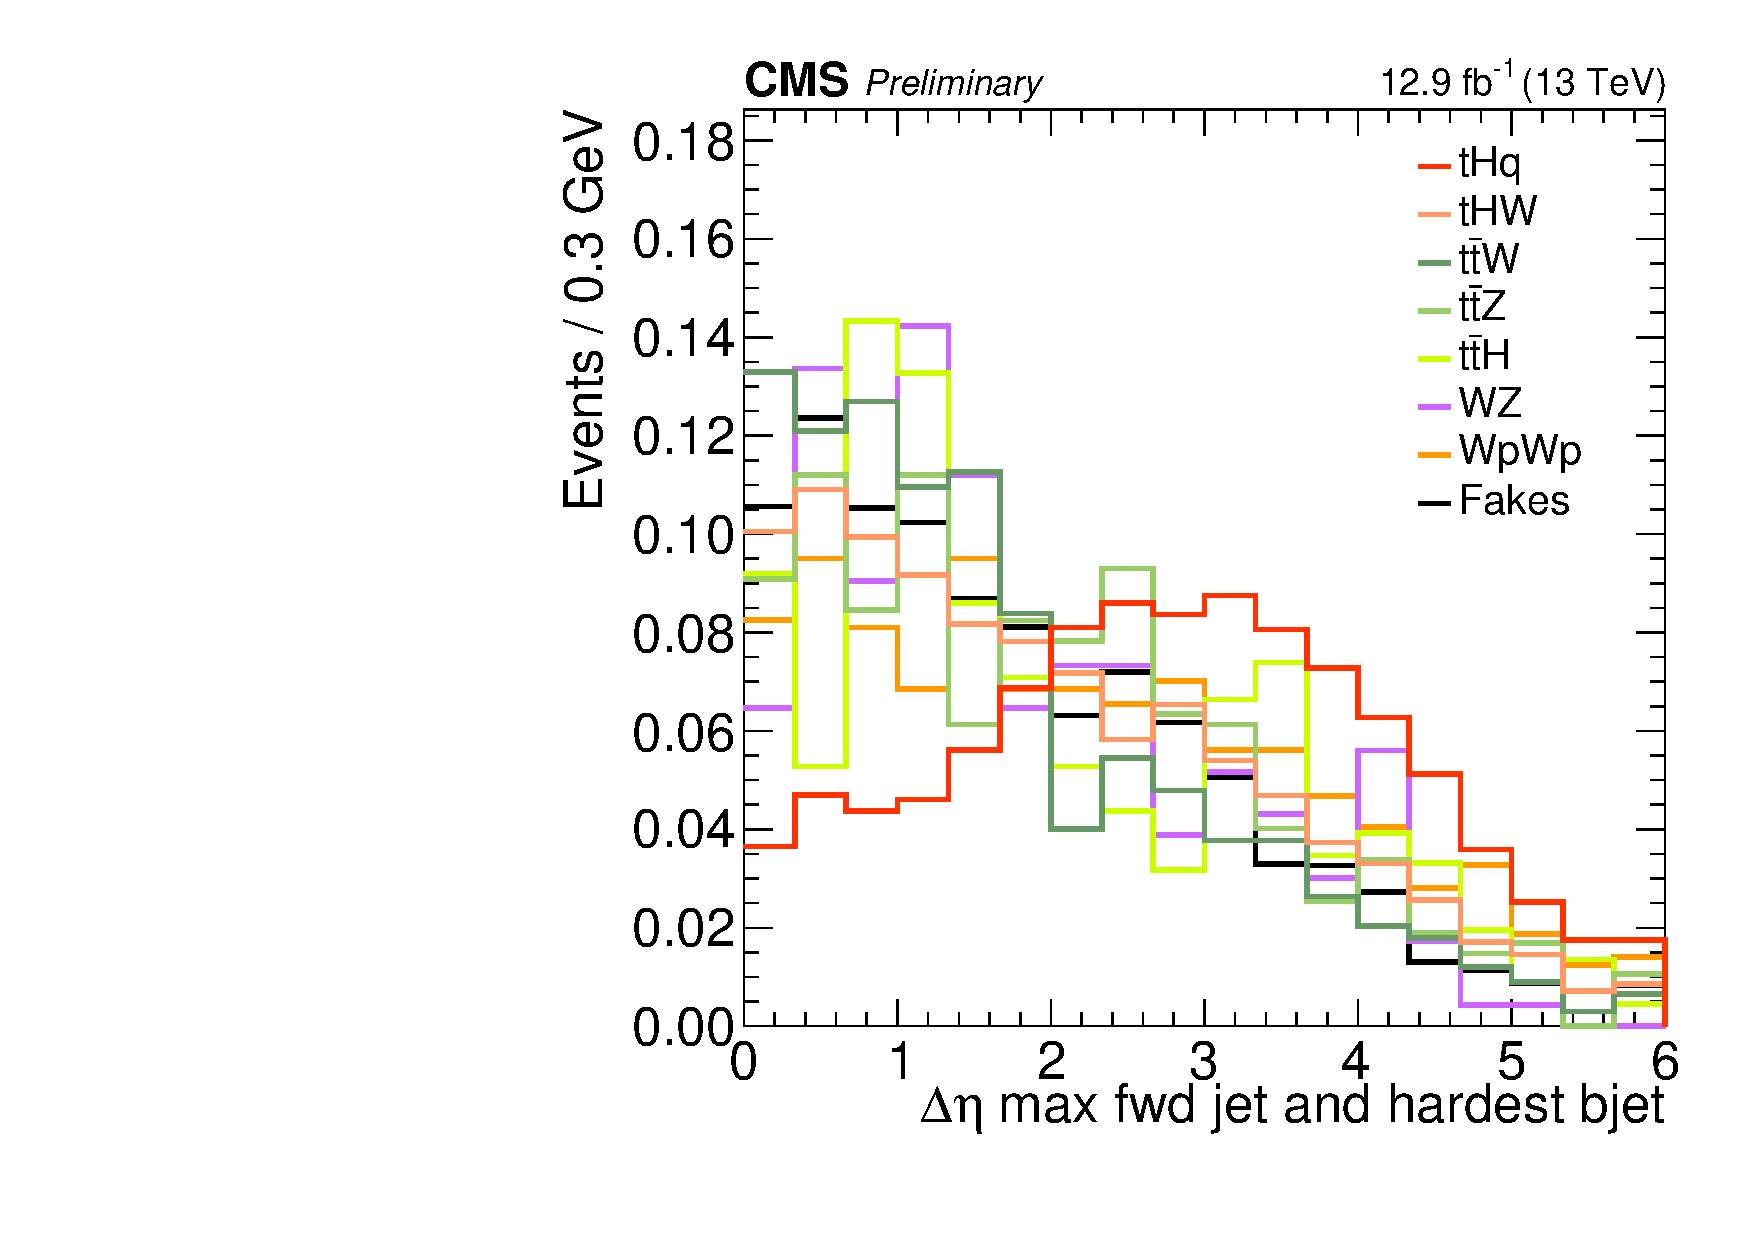
\includegraphics[width=0.32\textwidth]{dEtaFwdJetBJet_mumu.pdf}
  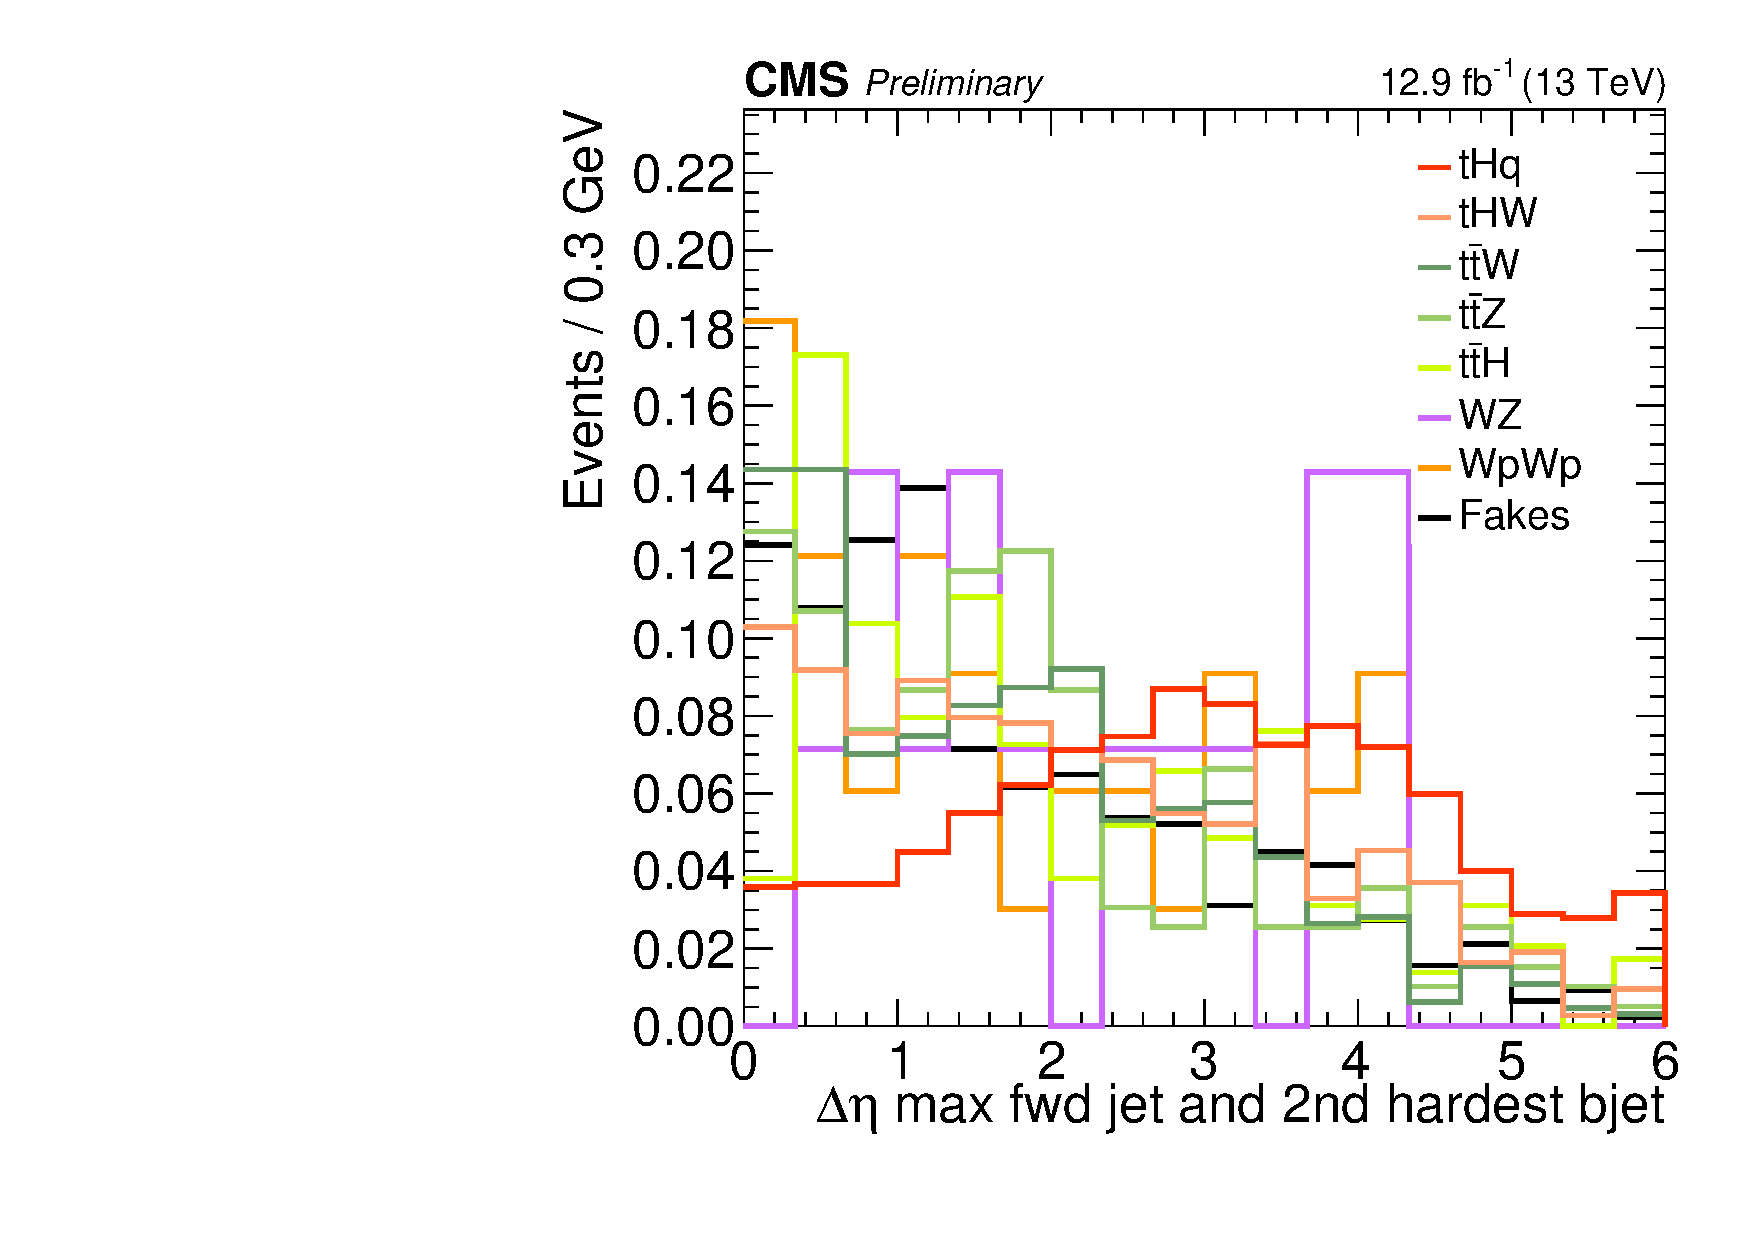
\includegraphics[width=0.32\textwidth]{dEtaFwdJet2BJet_mumu.pdf}\\
  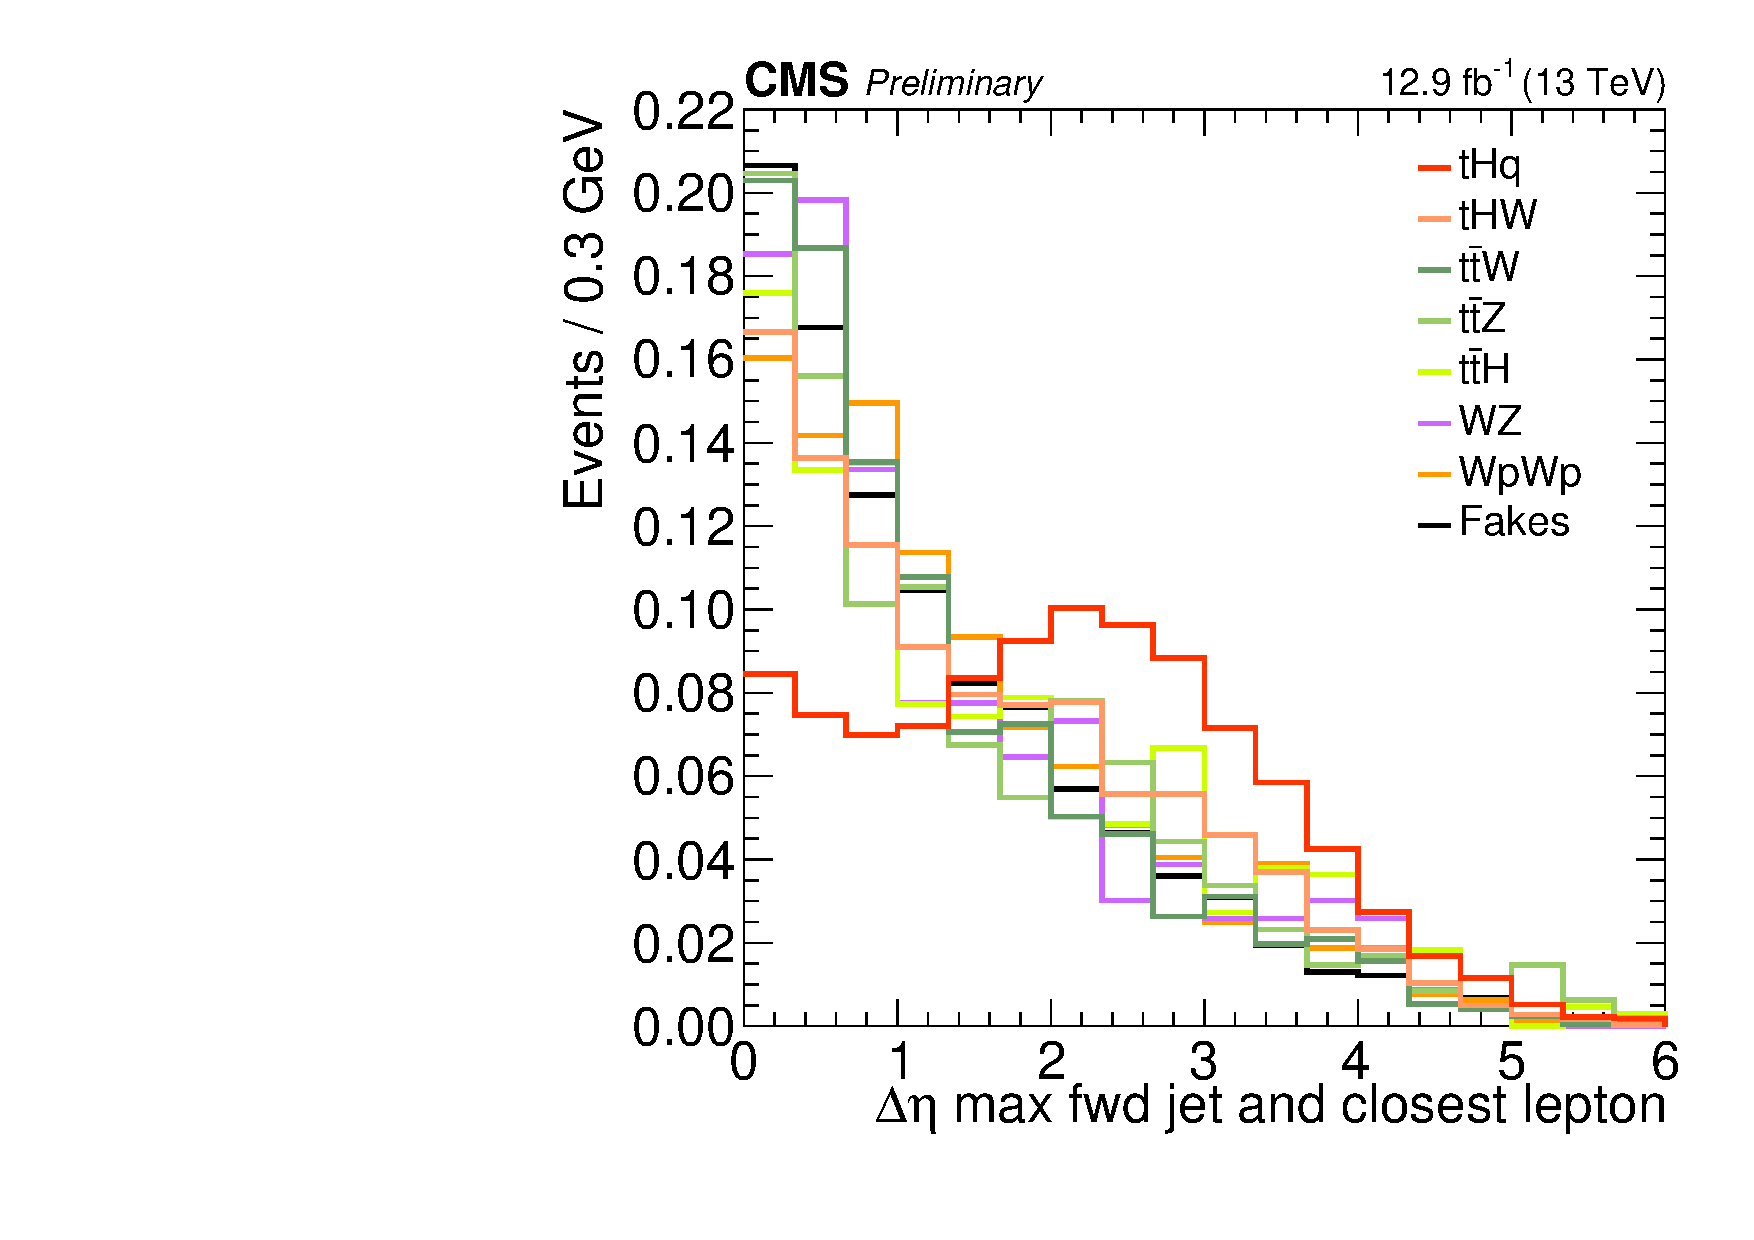
\includegraphics[width=0.32\textwidth]{dEtaFwdJetClosestLep_mumu.pdf}
  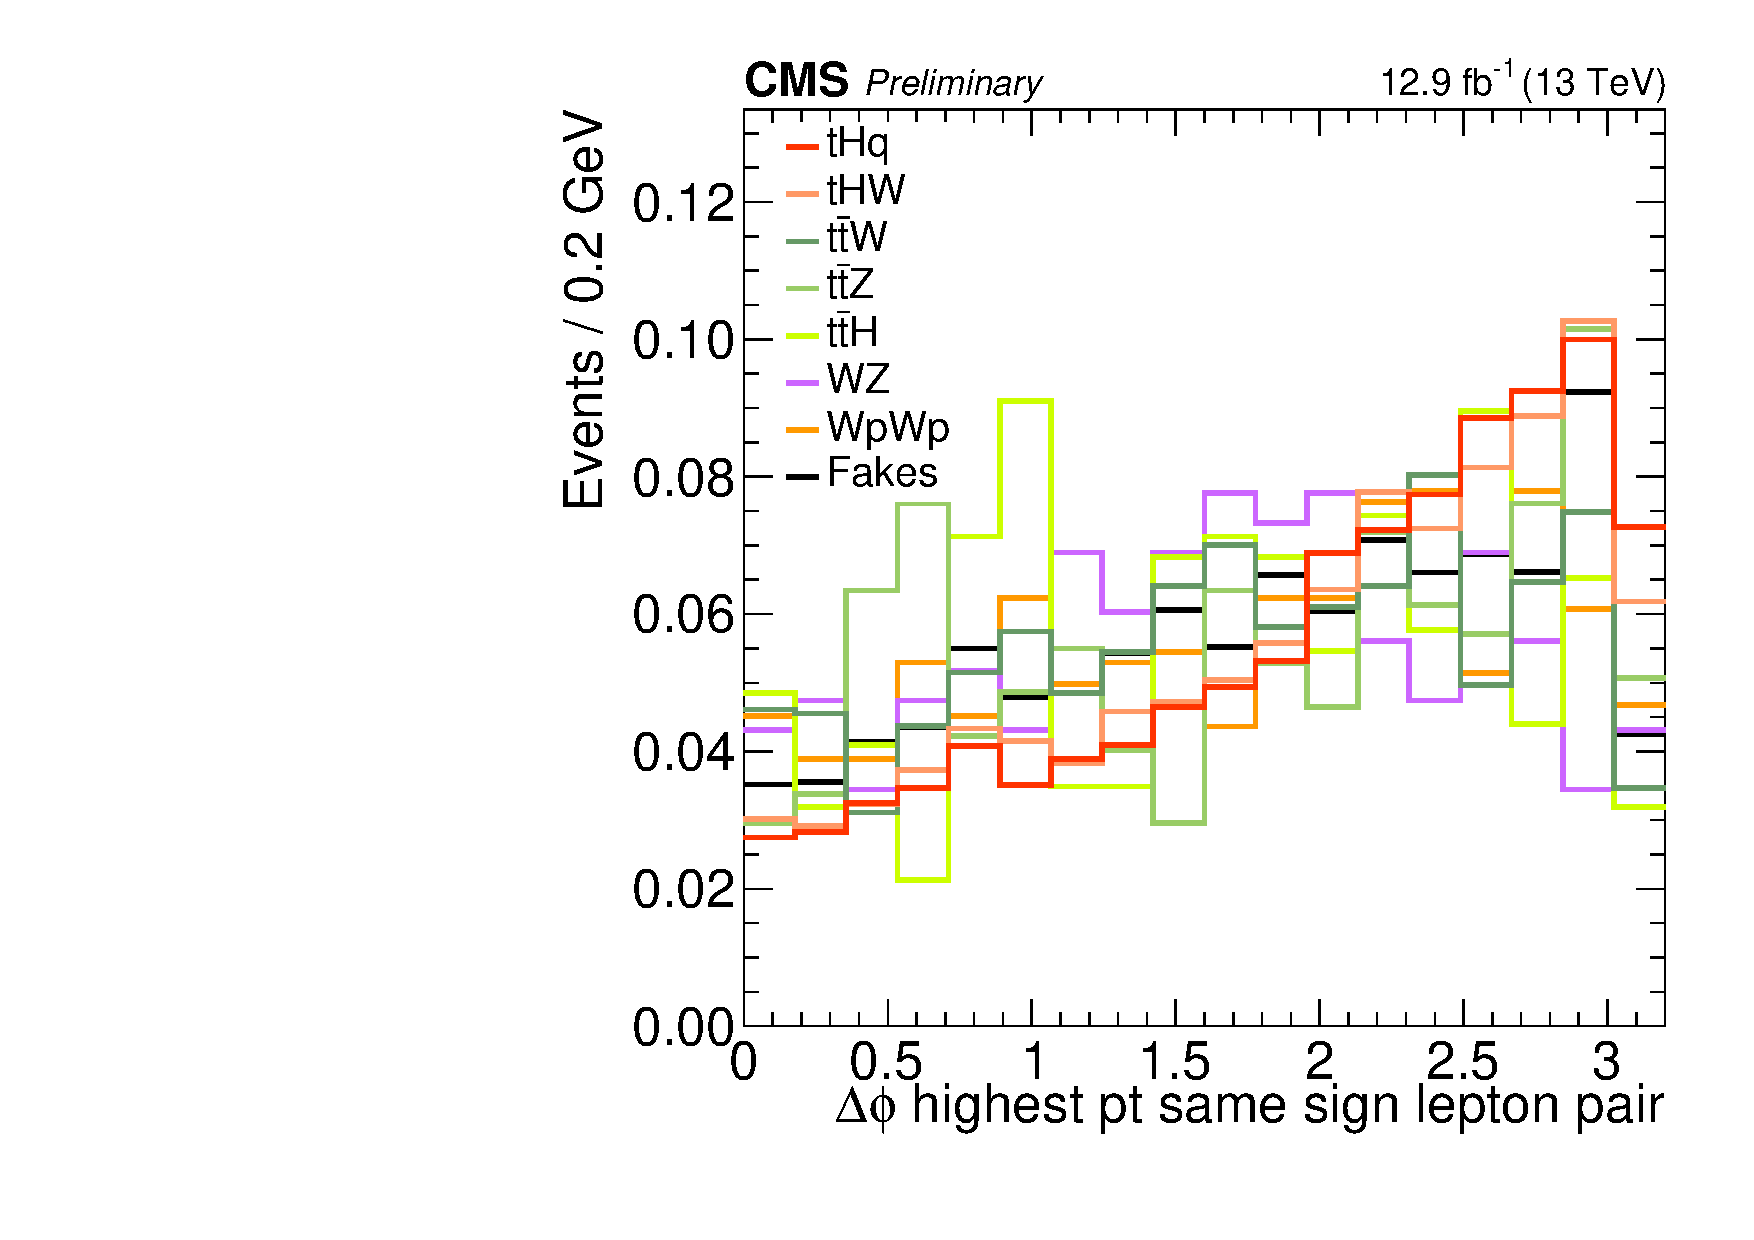
\includegraphics[width=0.32\textwidth]{dPhiHighestPtSSPair_mumu.pdf}
  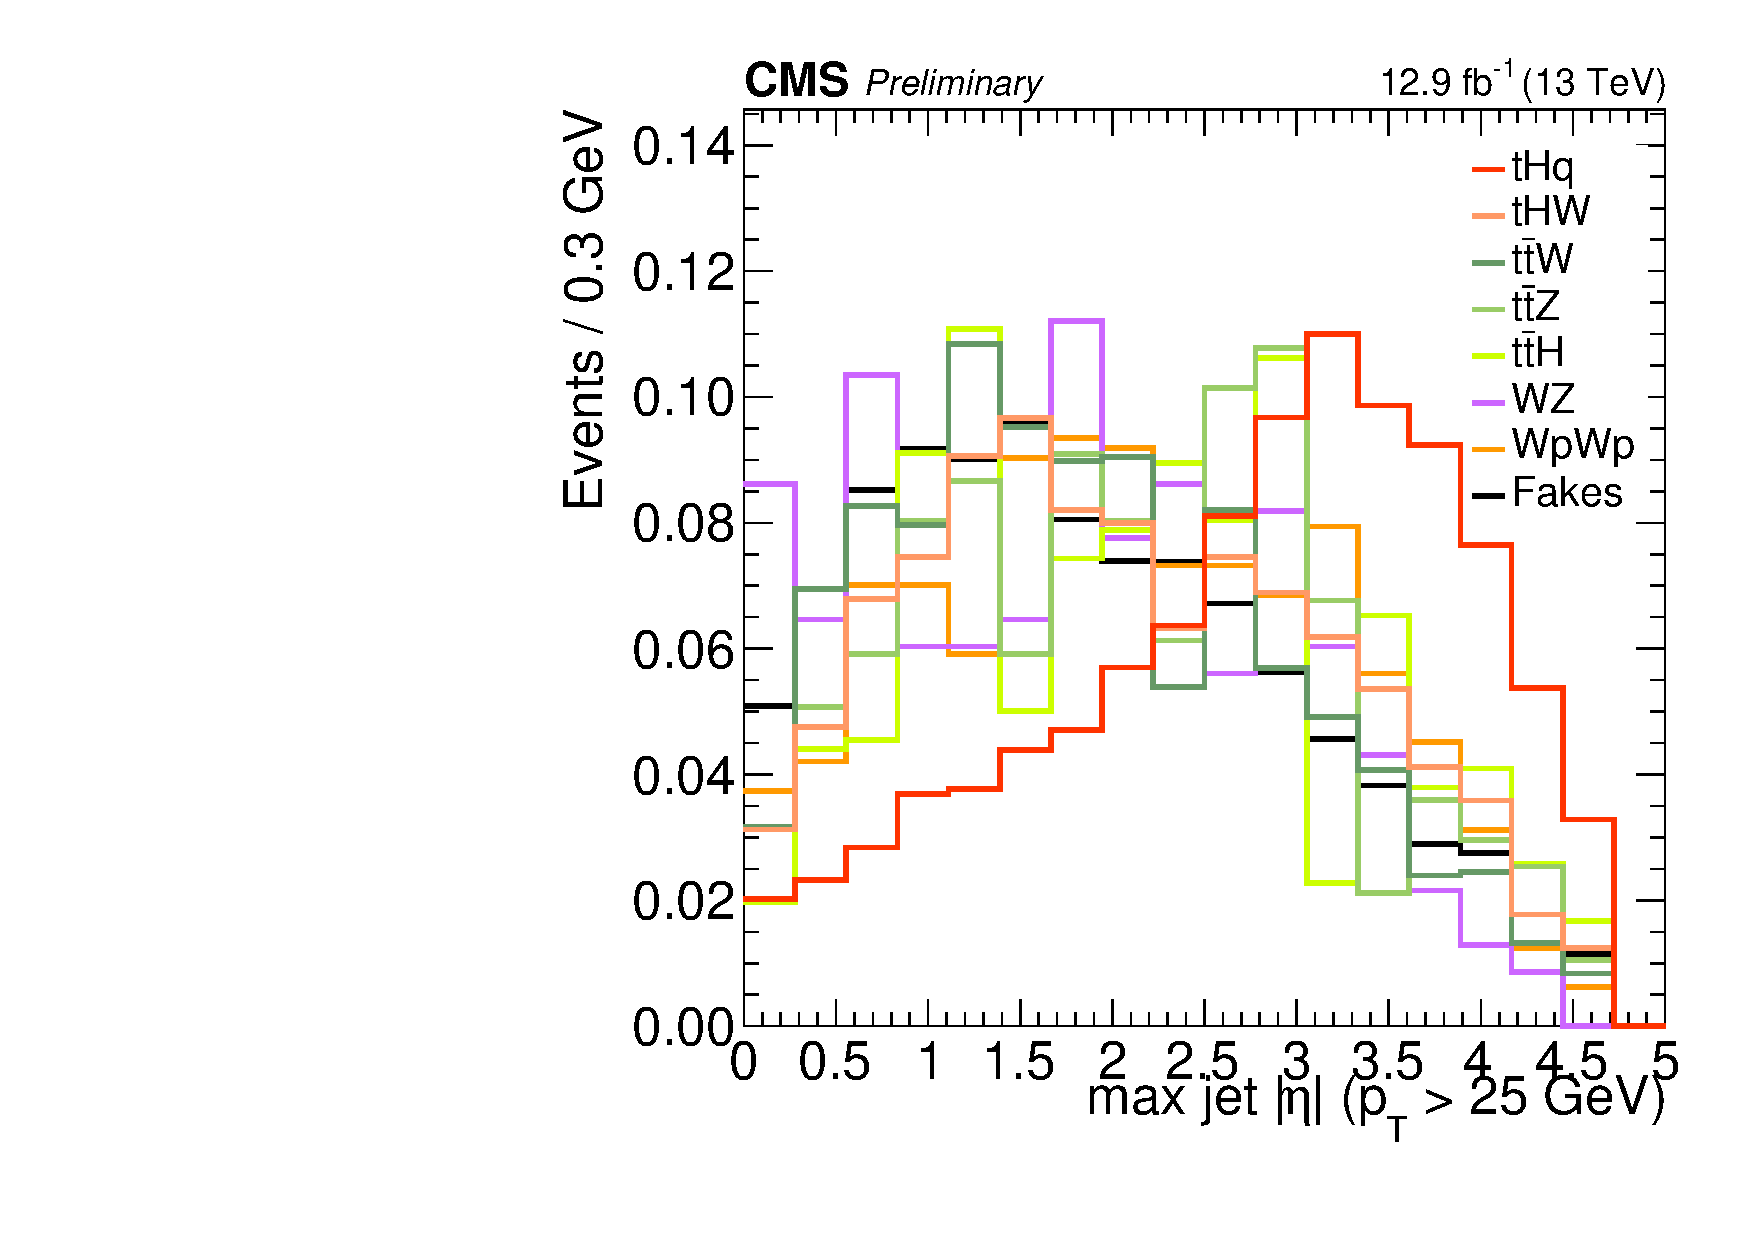
\includegraphics[width=0.32\textwidth]{maxEtaJet25_mumu.pdf}\\
  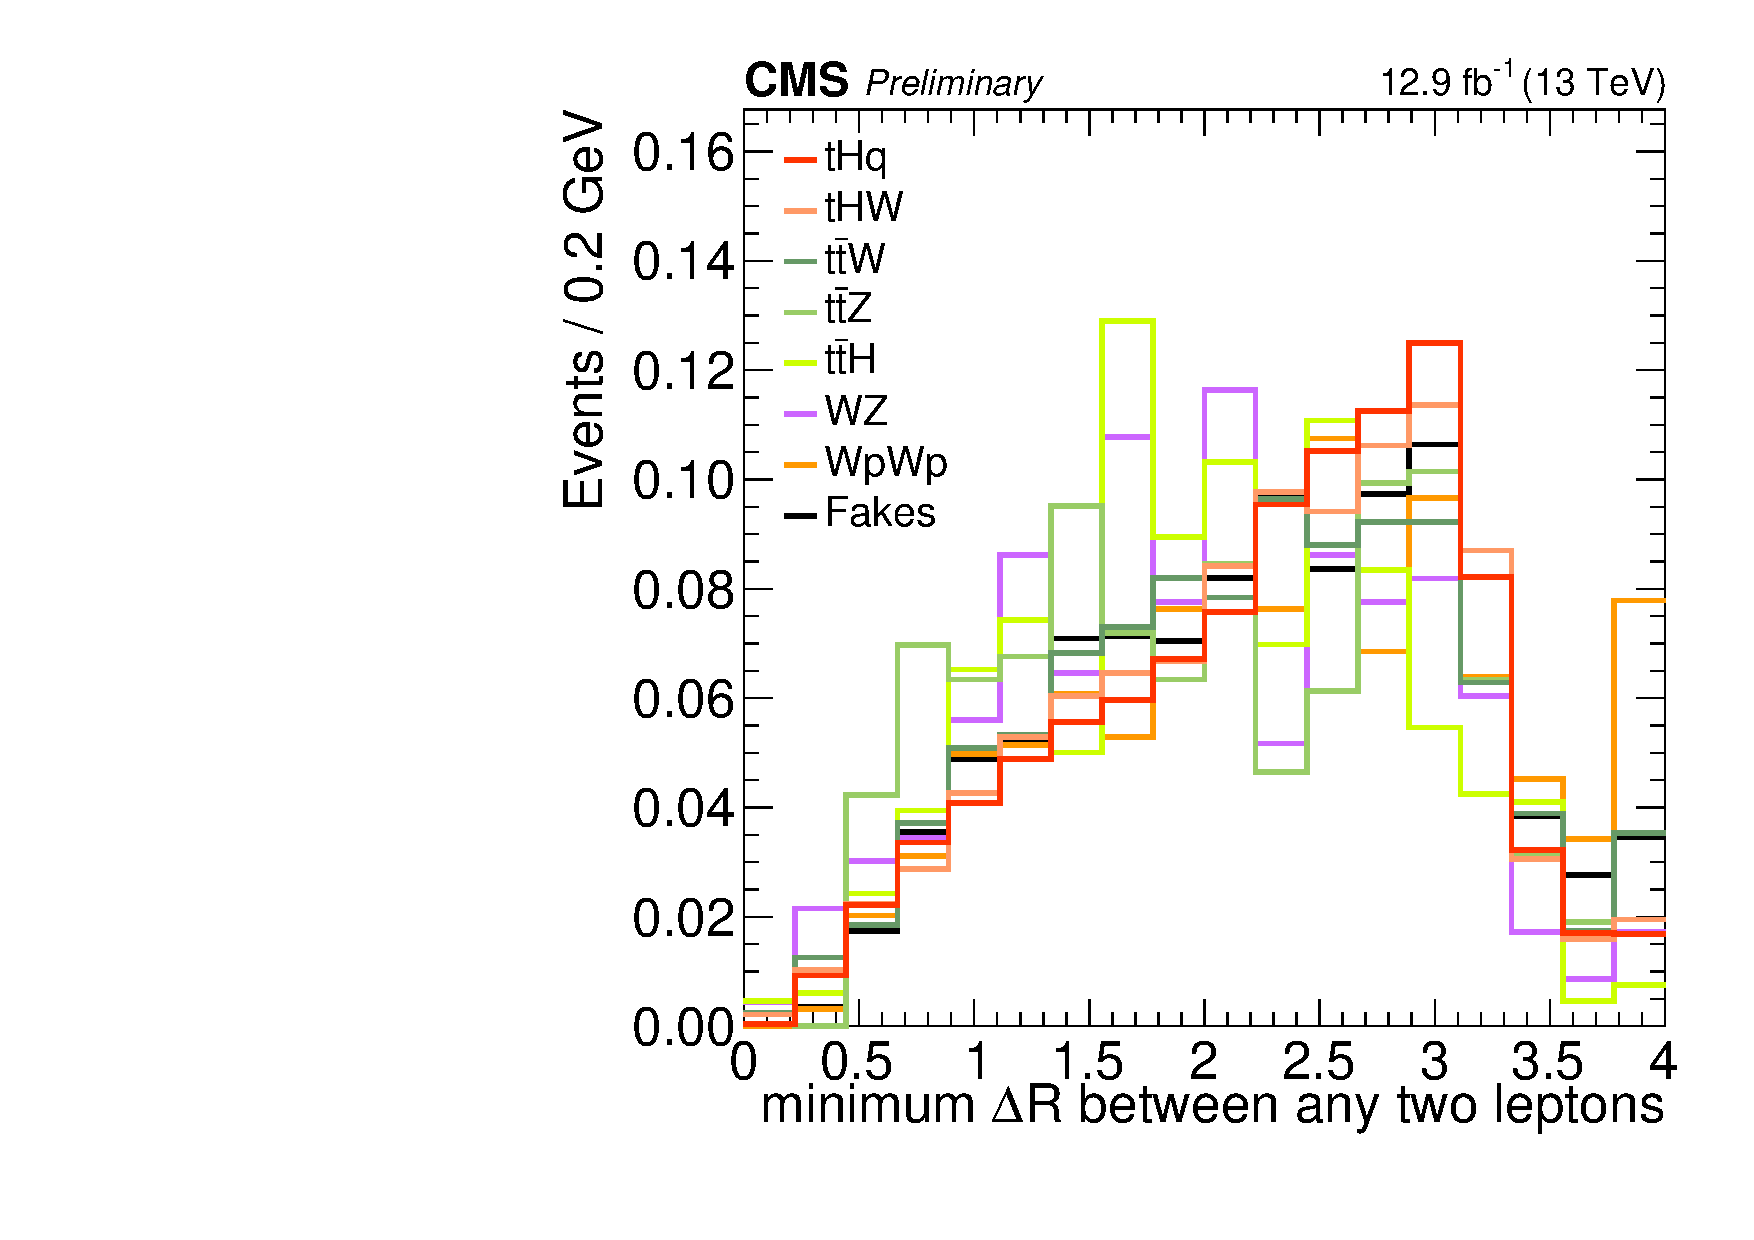
\includegraphics[width=0.32\textwidth]{minDRll_mumu.pdf}
  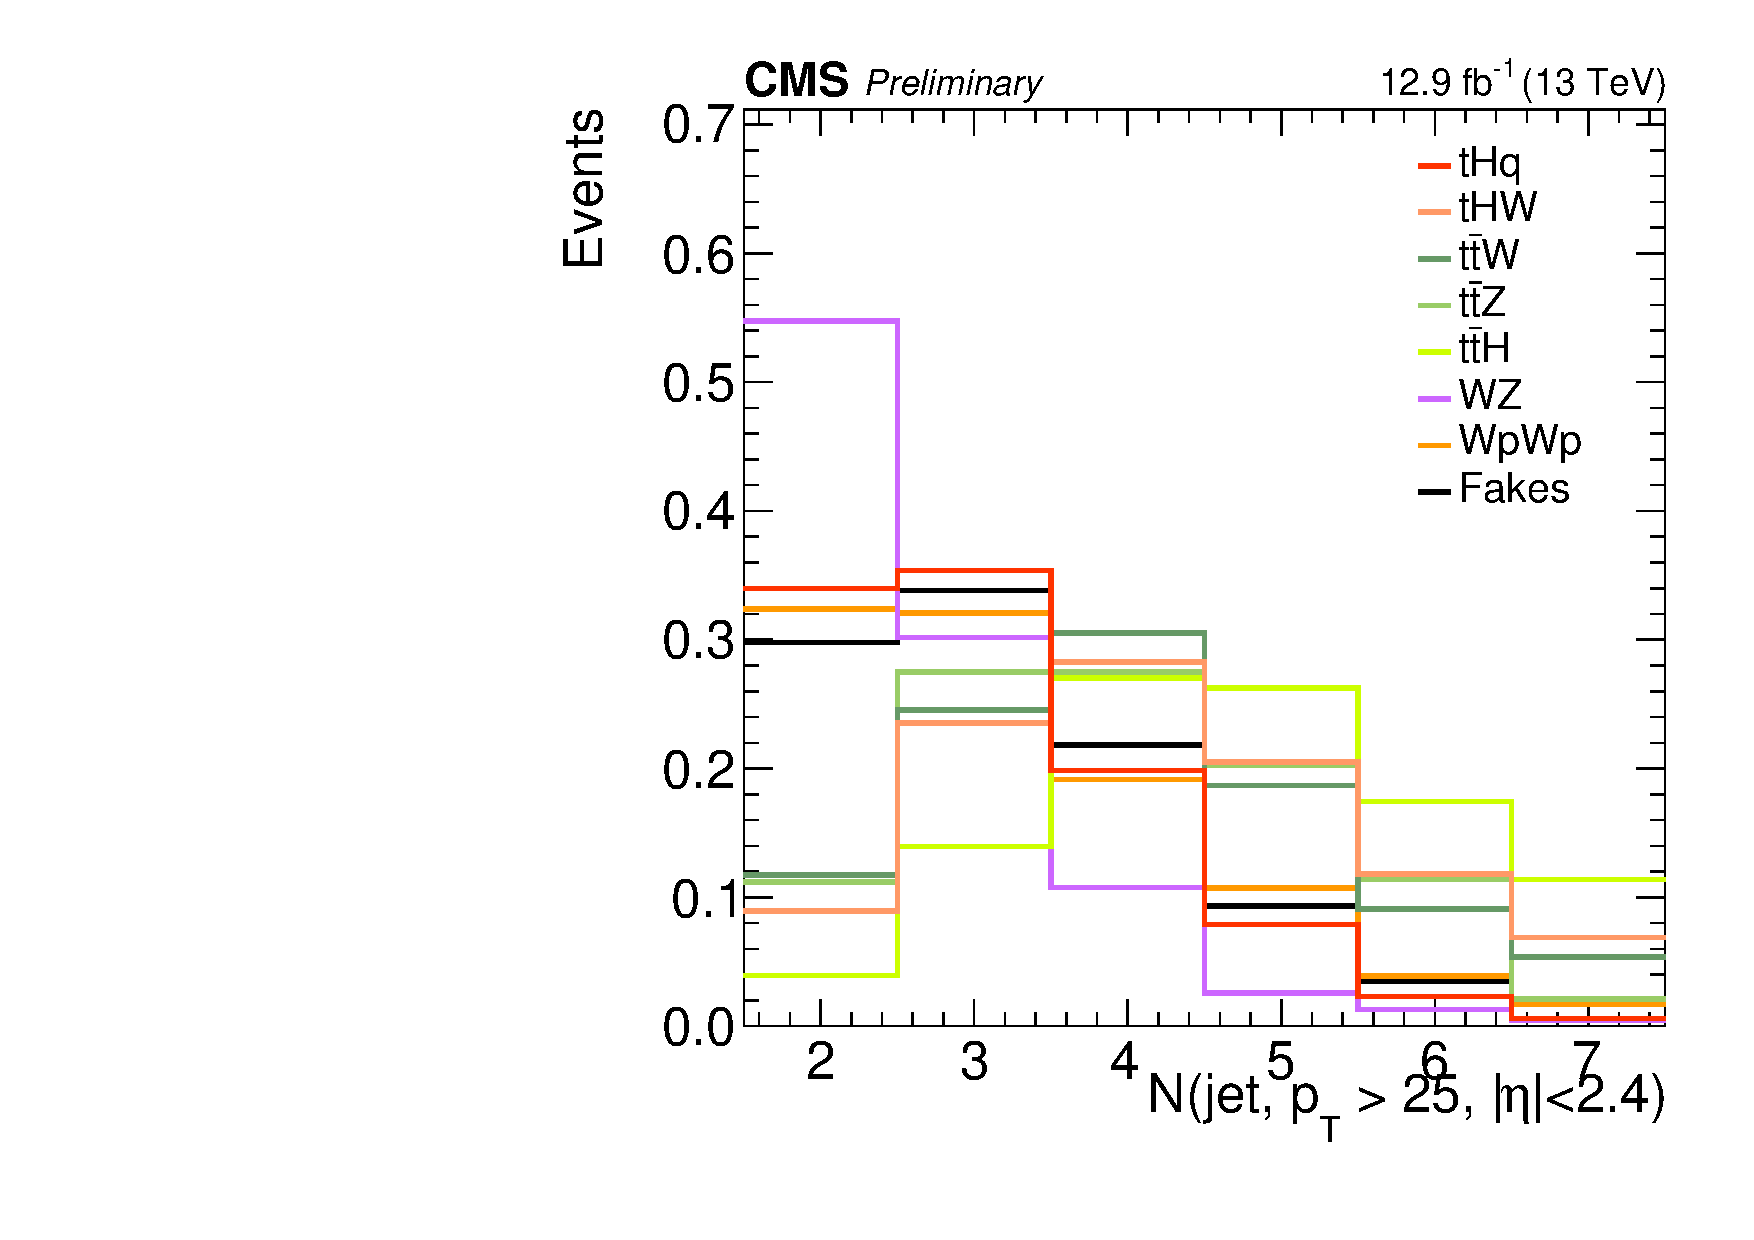
\includegraphics[width=0.32\textwidth]{nJet25_mumu.pdf}
  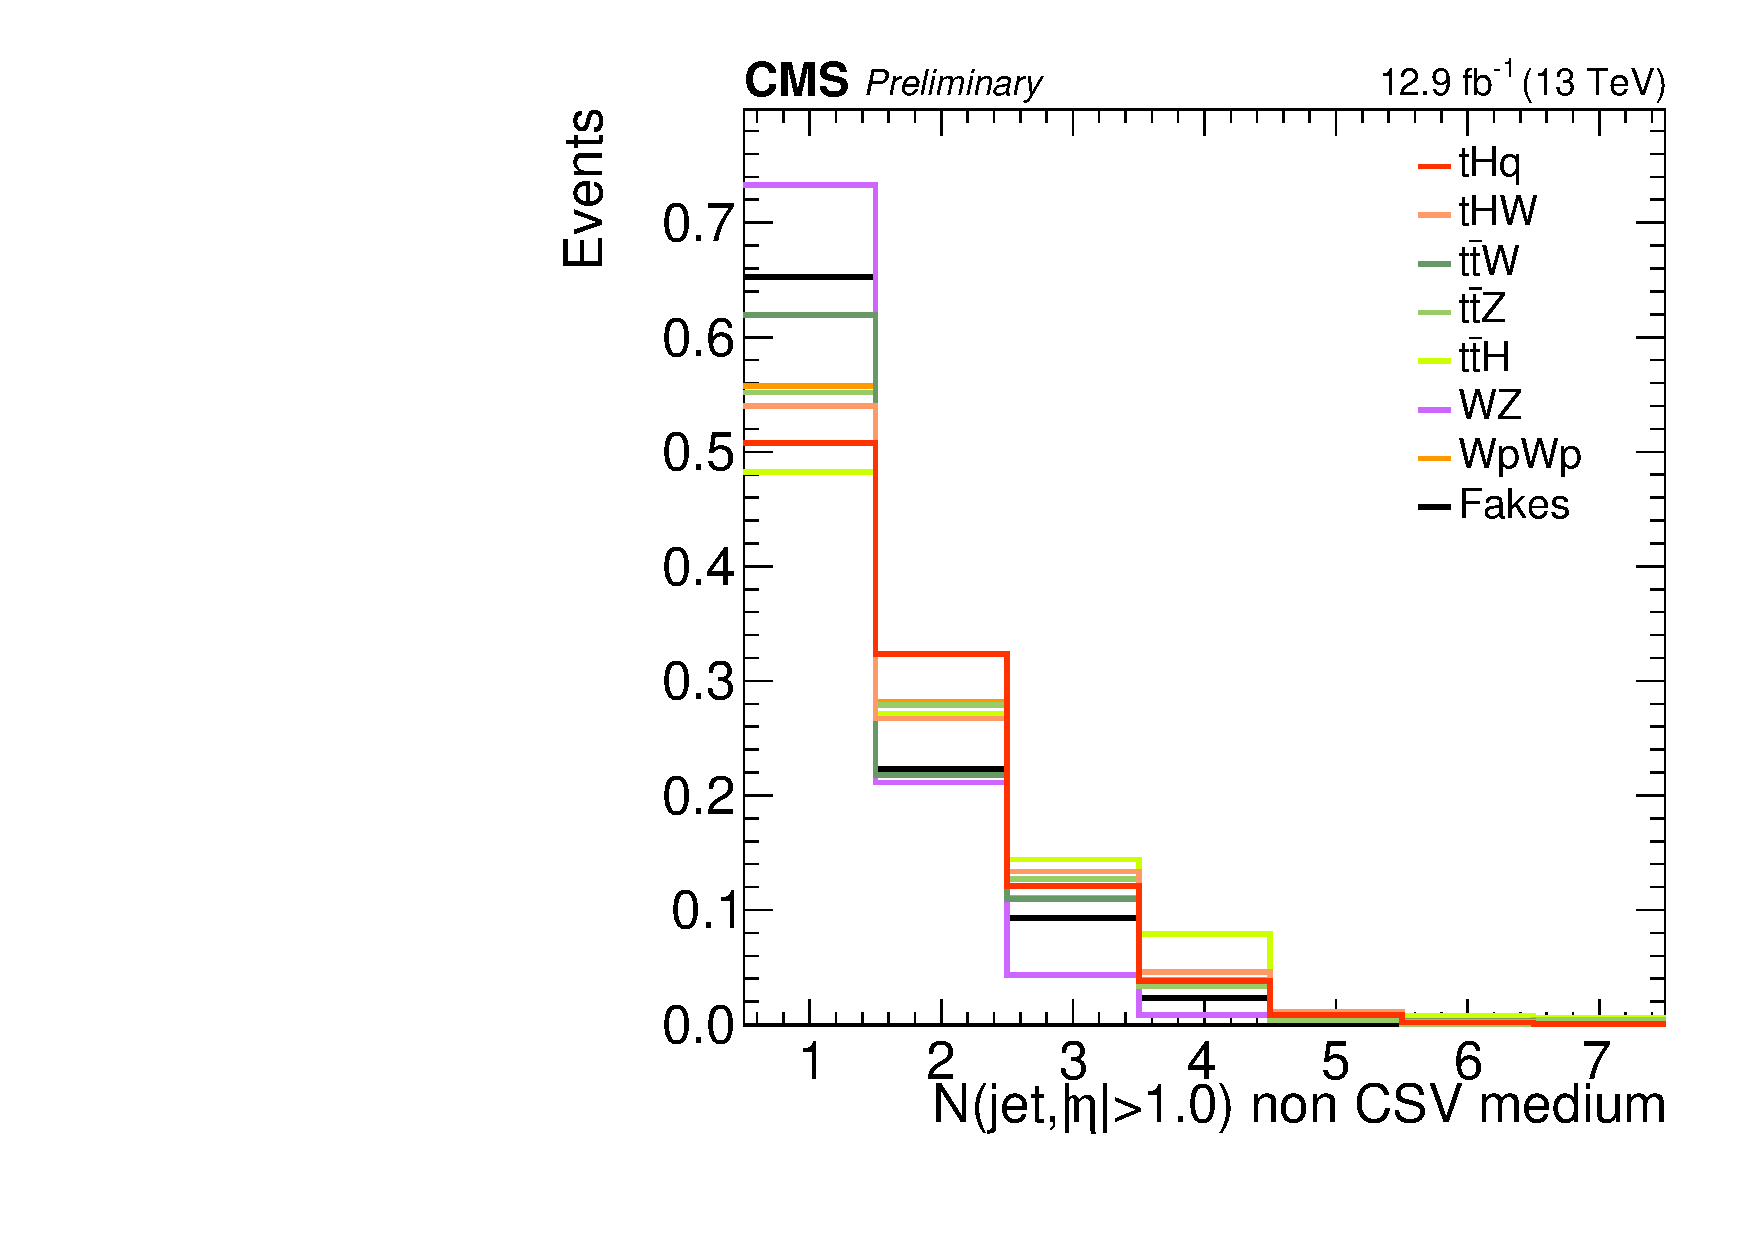
\includegraphics[width=0.32\textwidth]{nJetEta1_mumu.pdf}\\
  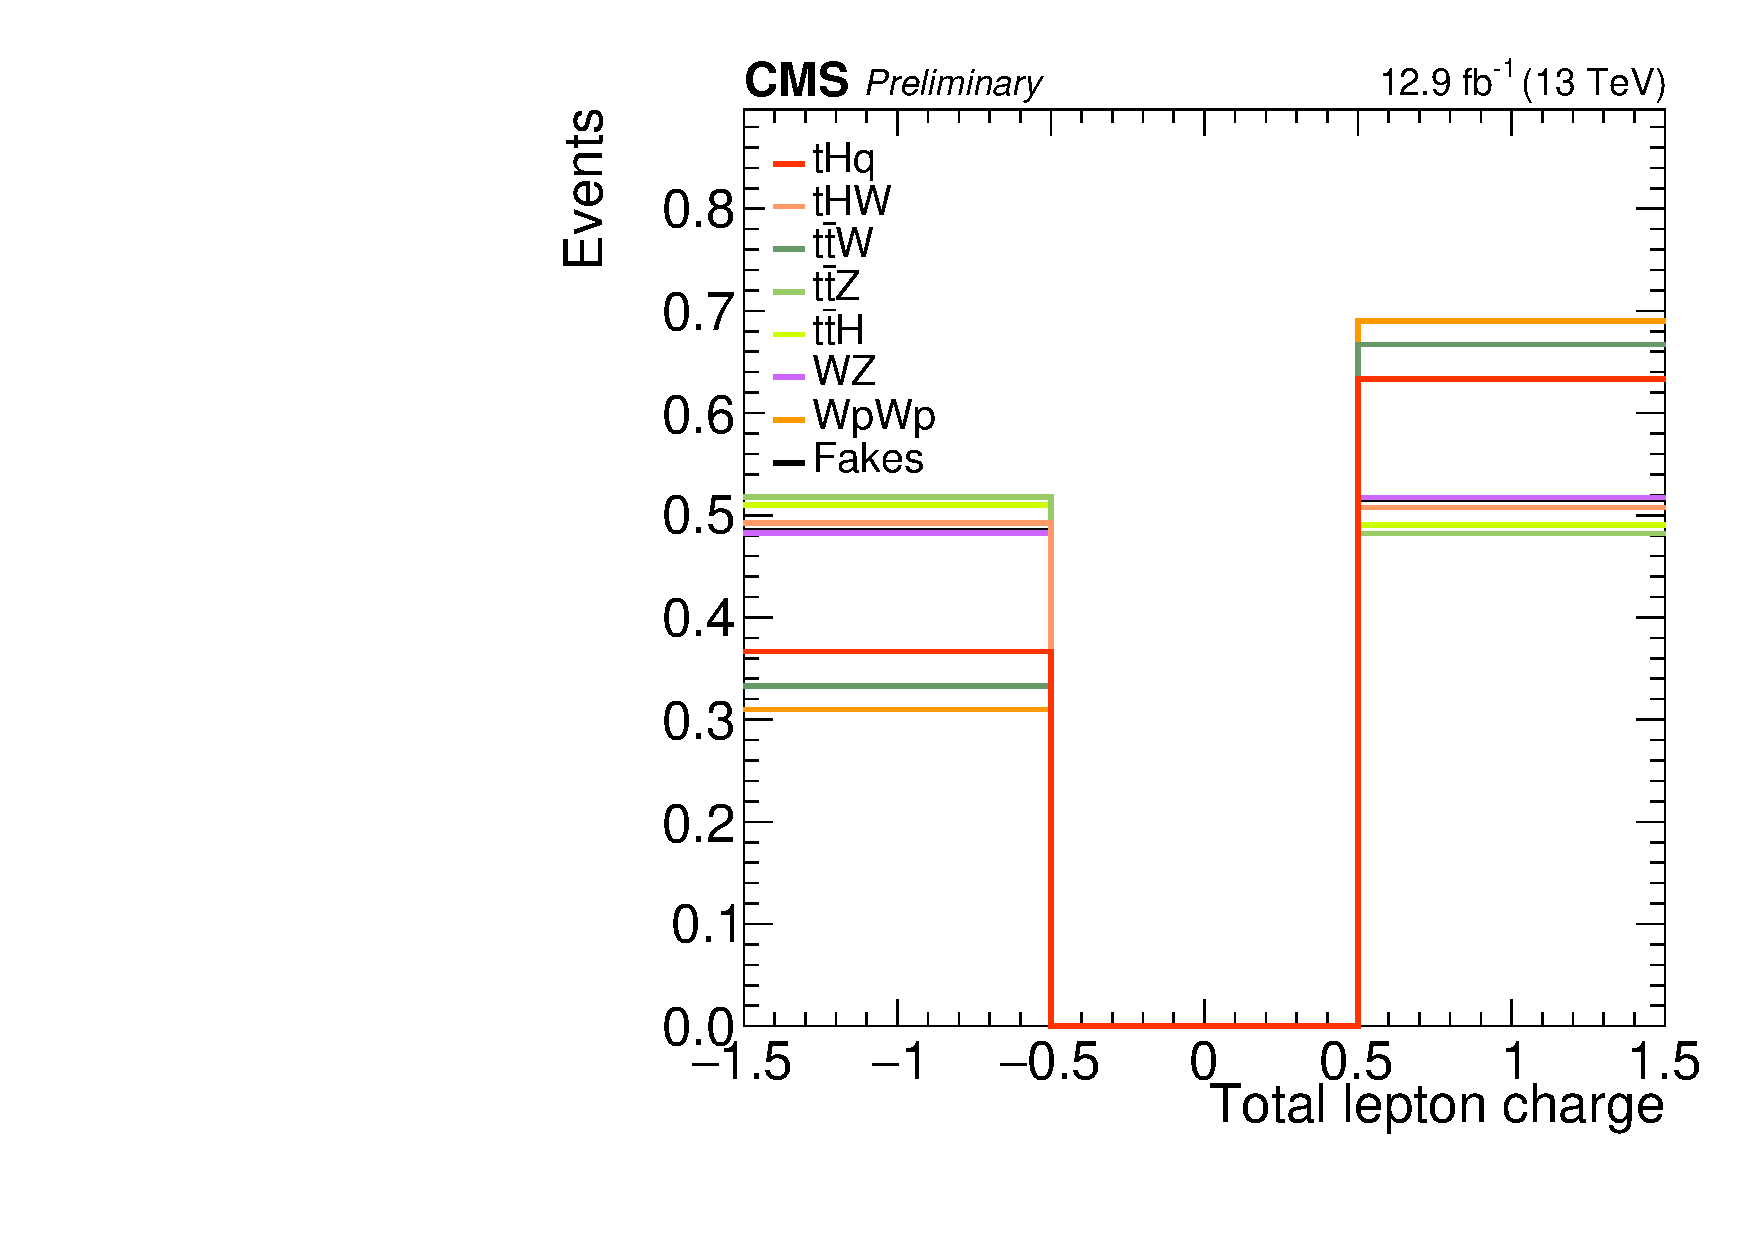
\includegraphics[width=0.32\textwidth]{totCharge_mumu.pdf}
  \caption[Input variables to the BDT, $2lss$ channel]{Distributions of input variables to the BDT for signal discrimination, normalized to the equal area, for the $2lss$ channel.}
  \label{fig:input_vars_2lss}
\end{figure}  

\newpage

\section{Input variables distributions from BDTG classifiers}

\begin{figure} [!h]
  \centering
  \includegraphics[width=\textwidth]{6var_tt.pdf}
  \includegraphics[width=0.66\textwidth]{4var_tt.pdf}
  \caption[BDT input variables. Discrimination against \ttbar\ in $2lss$ channel.]{BDT input variables as seen by BDTG classifier for the $2lss$ channel, \tHq signal (blue) discriminated against \ttbar\ background (red).}
  \label{mva_input_2lss_tt}
\end{figure}

\begin{figure} [!h]
  \centering
  \includegraphics[width=\textwidth]{6var_ttv.pdf}
  \includegraphics[width=0.66\textwidth]{4var_ttv.pdf}
  \caption[BDT input variables. Discrimination against \ttV\ in $2lss$ channel.]{BDT input variables as seen by BDTG classifier for the $2lss$ channel, \tHq signal(blue) discriminated against \ttV\ background (red).}
  \label{mva_input_2lss_ttv}
\end{figure}

\begin{figure} [!h]
  \centering
  \includegraphics[width=\textwidth]{mva_input1_tt.pdf}
  \includegraphics[width=\textwidth]{mva_input2_tt.pdf}
  \caption[BDT input variables. Discrimination against \ttbar in $3l$ channel.]{BDT input variables as seen by BDTG classifier for the $3l$ channel, \tHq signal (blue) discriminated against \ttbar\ background (red).}
  \label{mva_input_tt}
\end{figure}

\begin{figure} [!h]
  \centering
  \includegraphics[width=\textwidth]{mva_input1_ttv.pdf}
  \includegraphics[width=\textwidth]{mva_input2_ttv.pdf}
  \caption[BDT input variables. Discrimination against \ttV\ in $3l$ channel.]{BDT input variables as seen by BDTG classifier for the $3l$ channel, \tHq signal (blue) discriminated against \ttV\ background (red).}
\label{mva_input_ttv}
\end{figure}

\clearpage
\section{Pulls and impacts}\label{pulls_impacts_add}

\begin{figure} [!th]
  \centering
  
  \includegraphics[width=0.75\textwidth]{limits/impacts/impacts2.pdf}\\
  \includegraphics[width=0.75\textwidth]{limits/impacts/sm/impacts2.pdf}
  \caption[Additional post-fit pulls and impacts.]{Post-fit pulls and impacts of the next 20 nuisance parameters with largest impacts for the fit on the observed data, for the ITC (top) and SM (bottom) hypotheses. Continuation of pulls and impacts shown in Figure \ref{fig:impacts}}
  \label{fig:impacts2}
\end{figure}

  \begin{figure} [!h]
    \centering
    \includegraphics[width=0.75\textwidth]{limits/impacts/asimov/impacts2.pdf}\\
    \caption[Additional post-fit pulls an impacts for a fit to the Asimov dataset.]{Post-fit pulls and impacts of the next 20 nuisance parameters with largest impacts for a fit to the Asimov dataset with fixed signal strength, for the $\Ct/\CV=-1.0$ hypothesis. Continuation of pulls and impacts shown in Figure \ref{fig:impacts_asimov2}}
    \label{fig:impacts_asimov2}
  \end{figure}
